\documentclass[11pt,a4paper]{article}
\usepackage{amsmath,amssymb,calc,ifthen}
\usepackage{float}
%\usepackage{cancel}
\usepackage[table,usenames,dvipsnames]{xcolor} % for coloured cells in tables
\usepackage{tikz}
% Allows us to click on links and references!
\usepackage{hyperref}
\usepackage{url}
\hypersetup{
colorlinks,
citecolor=black,
filecolor=black,
linkcolor=black,
urlcolor=black
}
% Nice package for plotting graphs
% See excellent guide:
% http://www.tug.org/TUGboat/tb31-1/tb97wright-pgfplots.pdf
\usetikzlibrary{plotmarks,shapes}
\usepackage{amsmath,graphicx}
\usepackage{epstopdf}
\usepackage{caption}
\usepackage{subcaption}
\usepackage{graphicx}
% highlight - useful for TODOs and similar
\usepackage{color}
\newcommand{\hilight}[1]{\colorbox{yellow}{#1}}
\newcommand\ci{\perp\!\!\!\perp} % perpendicular sign
\newcommand*\rfrac[2]{{}^{#1}\!/_{#2}} % diagonal fraction
\newcommand\SLASH{\char`\\}
\usepackage{listings}
% margin size
\usepackage[margin=0.6in]{geometry}
\usepackage{pdfpages}
\usepackage{enumitem} % for nested enumerate numbers 1 1.1 1.1.1

\usepackage{titlesec} % reduce spacing after subsections
\usepackage{titling}

\setlength{\droptitle}{-5em}   % This is your set screw

% \titlespacing\subsection{0pt}{4pt plus 4pt minus 2pt}{4pt plus 2pt minus 2pt}


\begin{document}
\belowdisplayskip=12pt plus 3pt minus 9pt
\belowdisplayshortskip=7pt plus 3pt minus 4pt


% Hello dears, 
% 
% Ne pregatim sa facem programul pentru editia de anul acesta a Oxford for Romania. Ma bucur tare mult ca doriti sa va implicati ca lectori sau coordonatori de workshop si sper sa inspiram inca un grup de liceeni impreuna. 
% 
% Ca sa putem sa planificam mai bine, am sa va rog sa trimiteti o scurta propunere de curs pana pe data de 7 august. Nu trebuie sa fie mai mult de un A4, ne-am dori sa atinga urmatoarele puncte: 
% 
% 0. de ce credeti ca ar fi acest curs important pentru elevi
% 1. obiectivele cursului (SMART)
% 2. numarul minim de ore necesare si numarul ideal de ore
% 3. materialele de care aveti nevoie, e.g. proiector, markere, flipchart, internet, sala cu calculatoare si roboti, spaghetti :) s.a.m.d... 
% 4. experienta voastra in teaching (if any)
% 5. intervalul (ele) orare in care ati fi disponibili in perioada 27 aug- 1 septembrie
% 
% Daca ati participat si anul trecut si nu intentionati sa schimbati mare lucru la structura cursului, nu mai este nevoie sa raspundeti la acest email. Pentru cei care nu au participat, trimit cateva exemple de propuneri de anul trecut, poate sunt de ajutor. 
% 
% De asemenea, daca e vreo persoana din lista de lectori cu care considerati ca va puteti grupa (e.g. modulul Medical imaging- Neuroscience de anul trecut), ar fi minunat, pentru ca am asigura continuitatea si o mai buna sustinere a elevilor. 
% 
% Saptamana frumoasa, 


\title{Computer-generated 3D Graphics}

\author{Razvan V. Marinescu}

\vspace{-3em}
\maketitle

\section{Aim}

At the end of the course the students will:
\begin{itemize}
 \item Understand how 3D computer graphics is used in various industries
 \item Understand the benefits of using computer generated graphics (e.g. saving money) instead of more traditional forms of graphics (e.g. photos, movies)
 \item Be able to create simple 3D objects
 \item Be able to create a simple animation
 \item Be able to use lightning techniques to create more realistic images
 \item Know about the three main stages for creating a 3D object: modelling, texturing and rendering.
 \item Know how to apply these skills in their school projects, homeworks, etc ...
\end{itemize}


\section{Motivation}

This course is important for students because it introduces them to 3D computer-generated graphics, which is widely used in many industries such as:

\begin{figure}[H]
 \begin{subfigure}{0.31\textwidth}
 \centering
 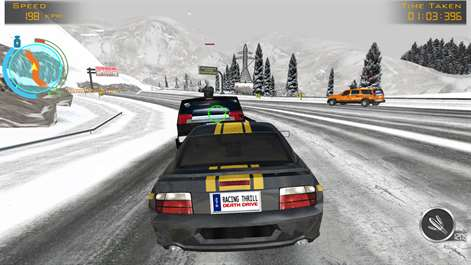
\includegraphics[height=80px,trim=20 0 20 0,clip]{images/racing_game.jpg}
 \caption{Computer games}
 \end{subfigure}
 \begin{subfigure}{0.31\textwidth}
 \centering
 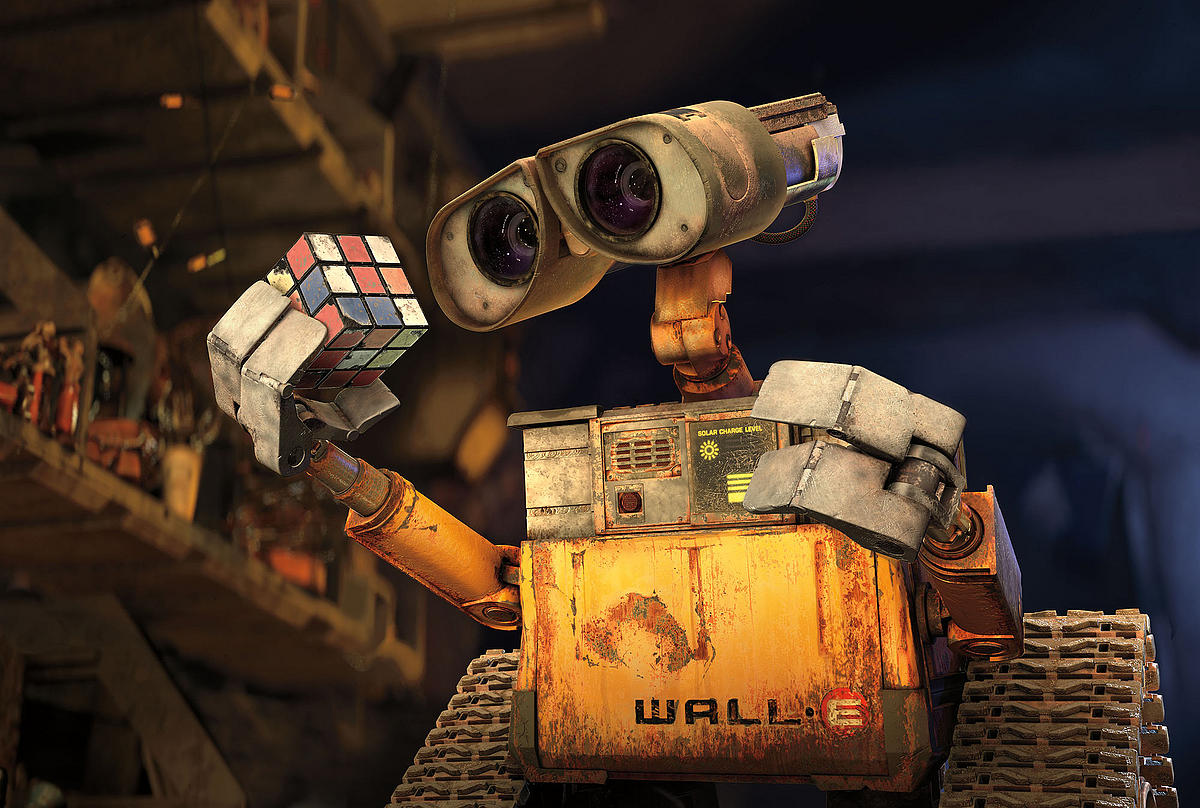
\includegraphics[height=80px]{images/walle}
 \caption{Animation films}
 \end{subfigure}
 \begin{subfigure}{0.31\textwidth}
 \centering
 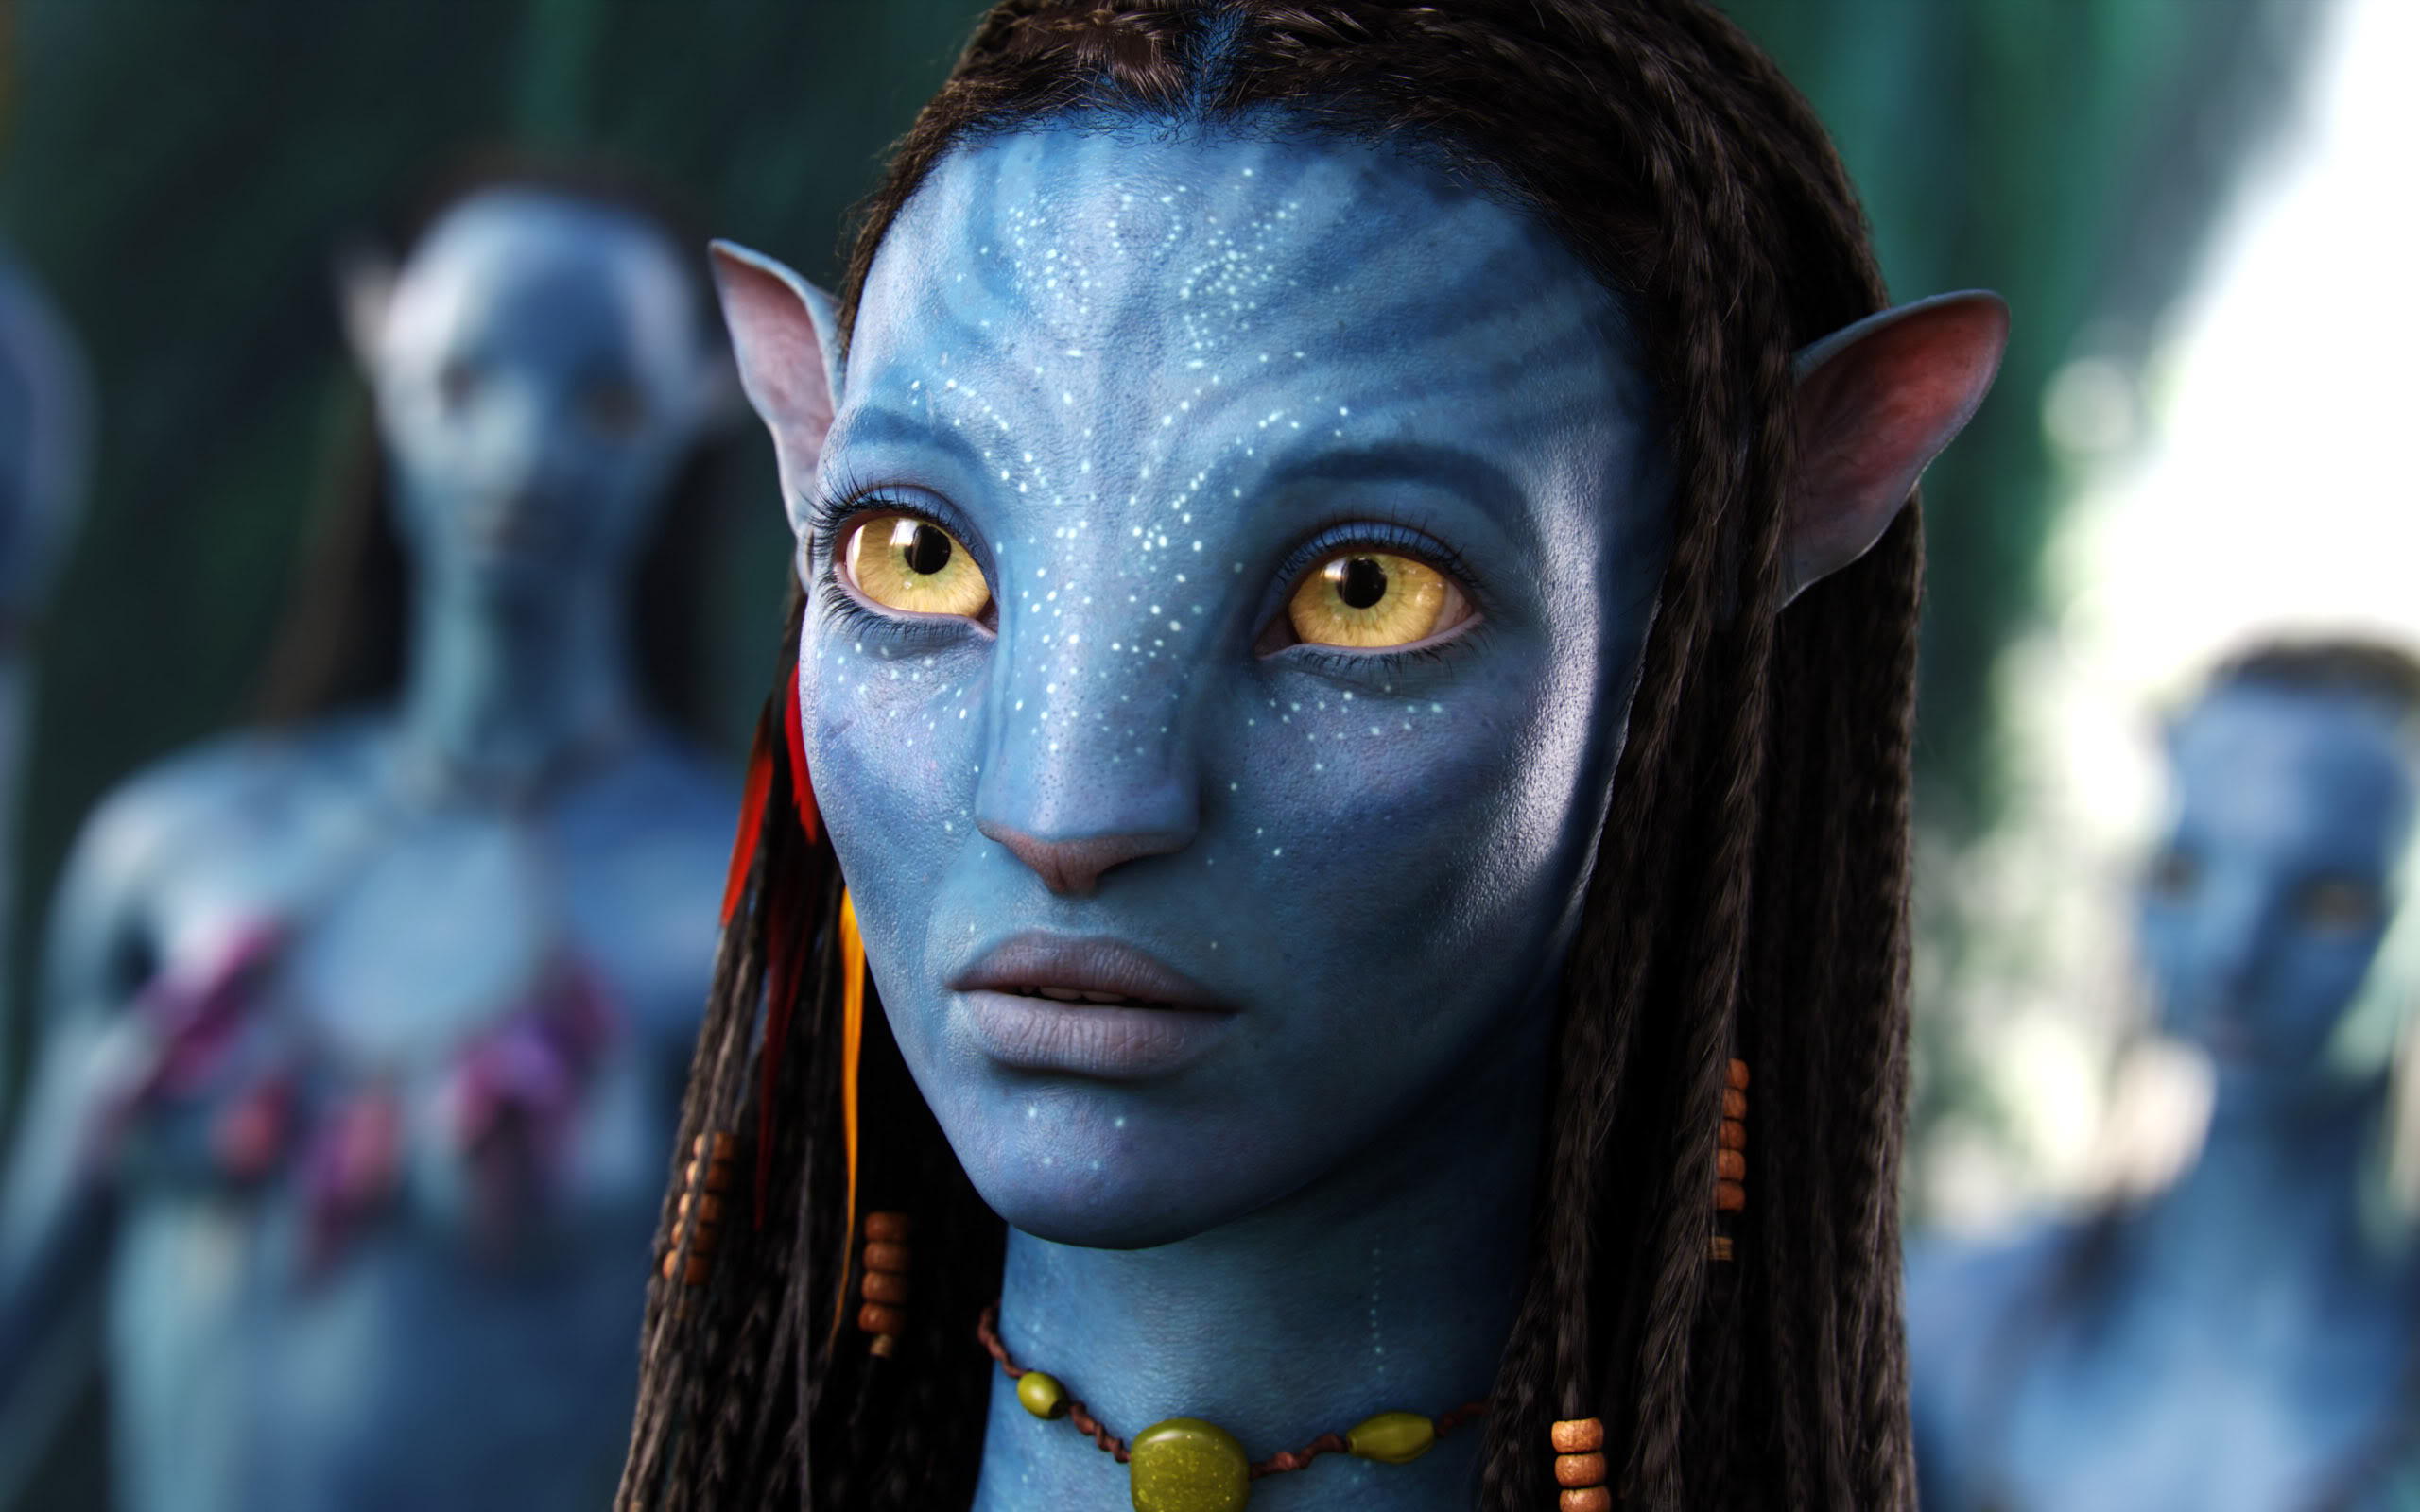
\includegraphics[height=80px]{images/avatar}
 \caption{Special effects in movies}
 \end{subfigure}
 \vspace{1em}
 
 \begin{subfigure}{0.31\textwidth}
 \centering
 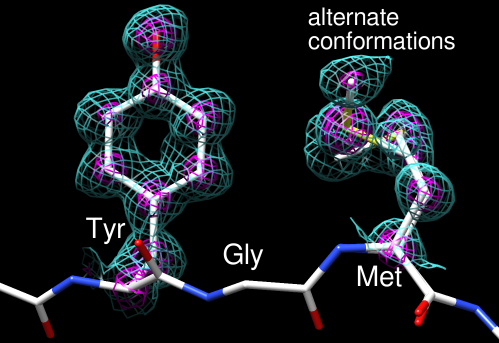
\includegraphics[height=80px]{images/molecular}
 \caption{Educational videos}
 \end{subfigure}
  \begin{subfigure}{0.31\textwidth}
  \centering
 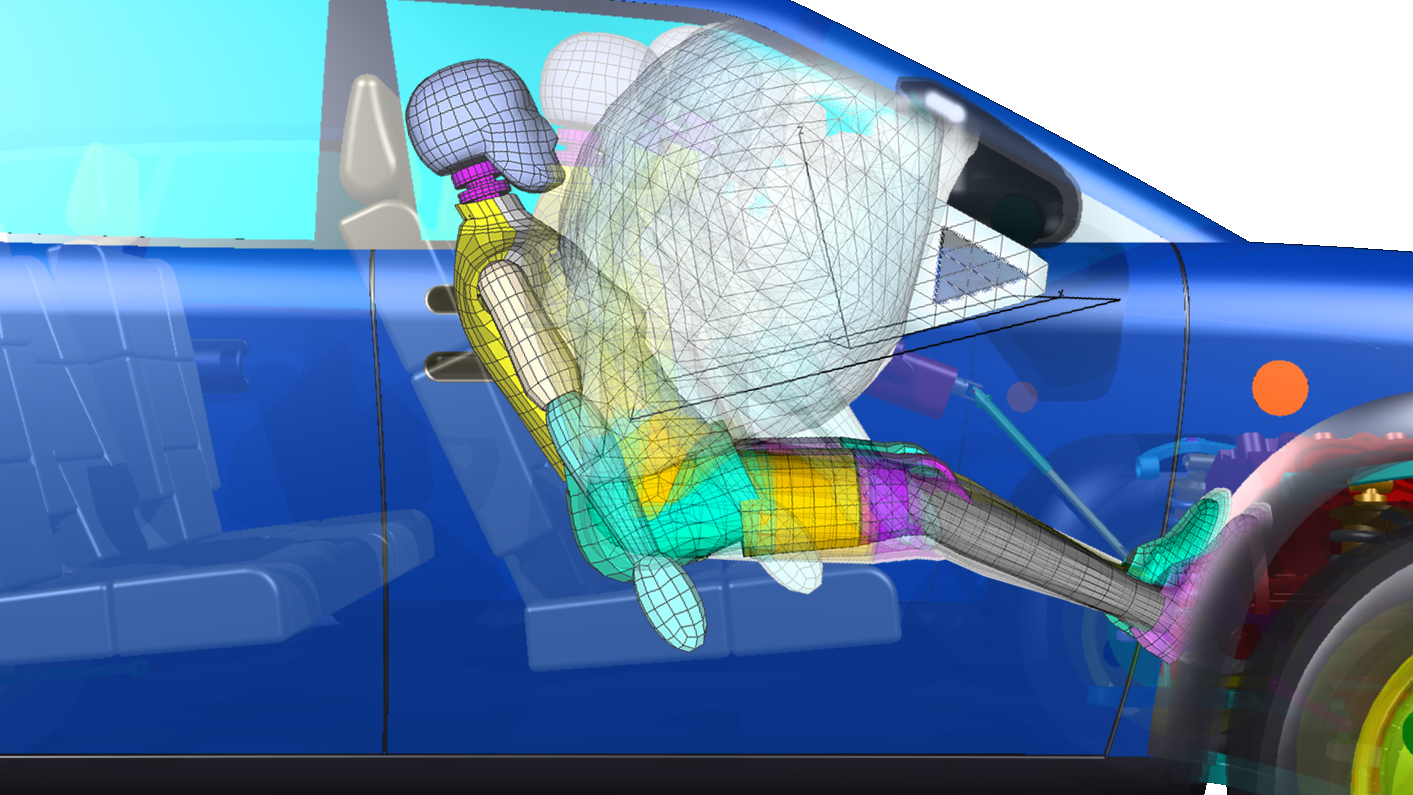
\includegraphics[height=80px,trim=100 0 100 0,clip]{images/car_crash}
 \caption{Simulations (e.g. car tests)}
 \end{subfigure}
   \begin{subfigure}{0.31\textwidth}
   \centering
 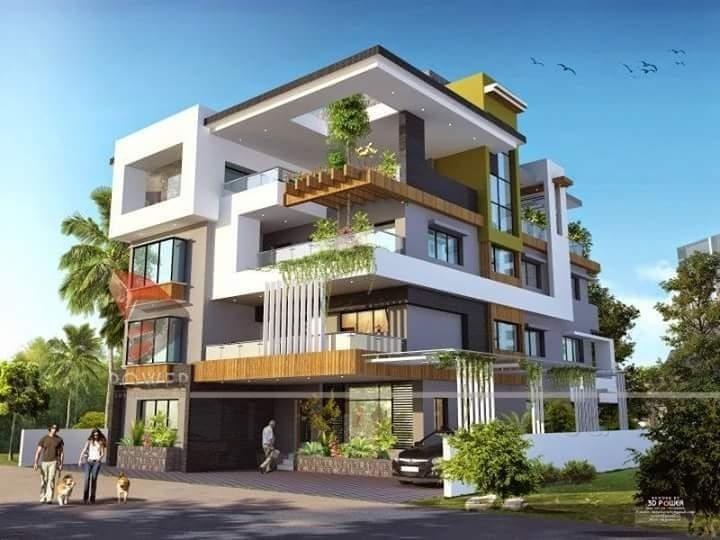
\includegraphics[height=80px]{images/building_design.jpg}
 \caption{Architecture design}
 \end{subfigure}
  \vspace{1em}
 
  \begin{subfigure}{0.31\textwidth}
  \centering
 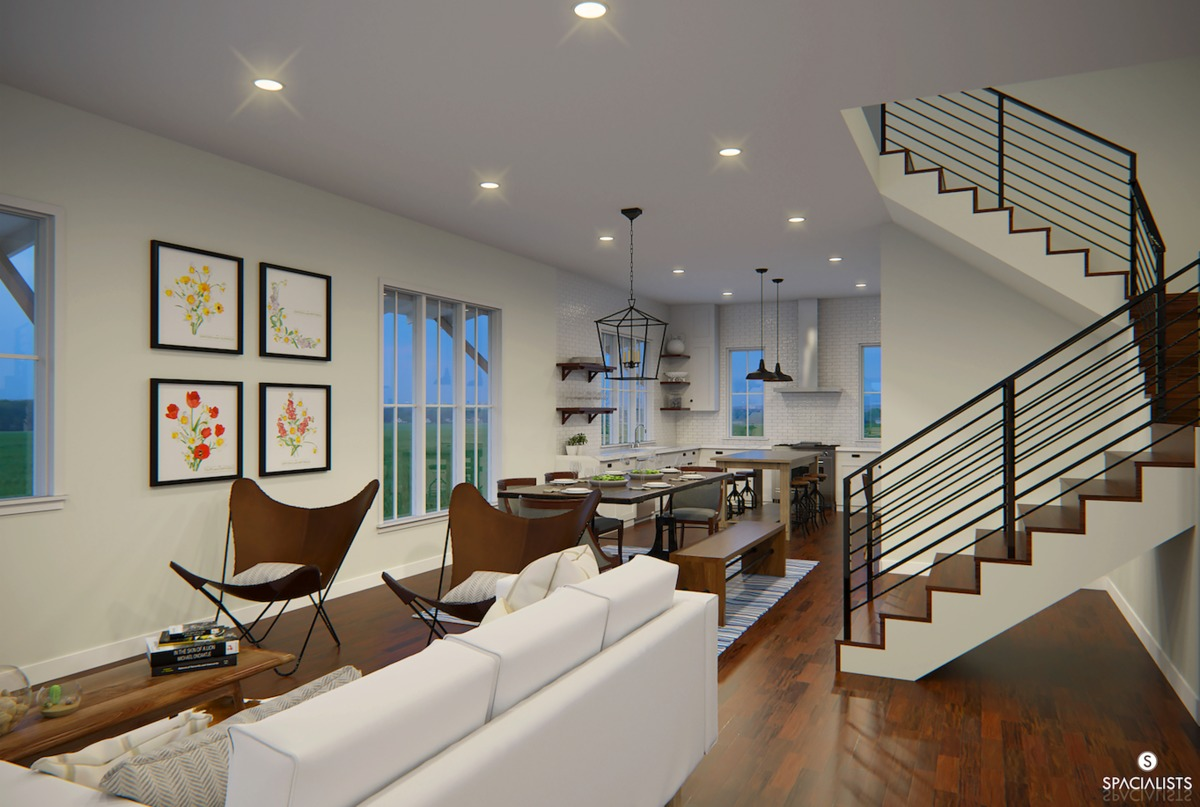
\includegraphics[height=80px]{images/interior_design.jpg}
 \caption{Interior design}
 \end{subfigure}
  \begin{subfigure}{0.31\textwidth}
  \centering
 
\includegraphics[height=80px]{images/advertisement.jpg}
 \caption{Advertisements}
 \end{subfigure}
   \begin{subfigure}{0.31\textwidth}
   \centering
 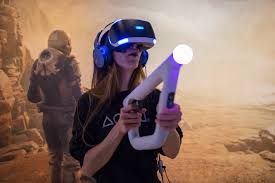
\includegraphics[height=80px]{images/virtual_reality.jpg}
 \caption{Virtual Reality}
 \end{subfigure}
 \caption{The industries where 3D computer-generated graphics is used}
 \label{fig:ind}
\end{figure}

The students will be able to assess whether they like this kind of work and perhaps consider one of these industries as their career options. Furthermore, the skills learned in this course can also aid students in their school projects or homeworks, as it enables them to make realistic 3D models of any object they like. These drawings will add a lot of value to reports and presentations they will make in school, university and later on at their workplace.


\section{Lesson Plan}

\subsection{Presentation: Overview of 3D Computer Graphics - 20 min}


% The students will be explained what 3D graphics is and how it is currently used in several industries:
% \begin{itemize}
%  \item Computer games
%  \item Animations 
%  \item Special effects in movies
%  \item Educational videos (e.g. showing molecular interactions)
%  \item Simulations (e.g. car crash tests)
%  \item Architecture and interior design
%  \item Advertisements
%  \item Virtual Reality
% \end{itemize}
I will explain what computer-generated graphics is and how it is used currently in many industries (Fig. \ref{fig:ind}). We will then discuss the motivations for using computer generated graphics in each industry (i.e. save money, generate images not otherwise available in the real world). I will then explain the three key stages for creating a 3D computer-generated object: Modelling, Texturing and Rendering.
% \begin{itemize}
%  \item Modelling
%  \item Texturing
%  \item Animating
%  \item Rendering
% \end{itemize}

\begin{figure}[H]
 \begin{subfigure}{0.31\textwidth}
 \centering
 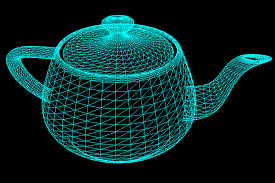
\includegraphics[height=80px,trim=20 0 20 0,clip]{images/teapot_modelling}
 \caption{Modelling}
 \end{subfigure}
 \begin{subfigure}{0.31\textwidth}
 \centering
 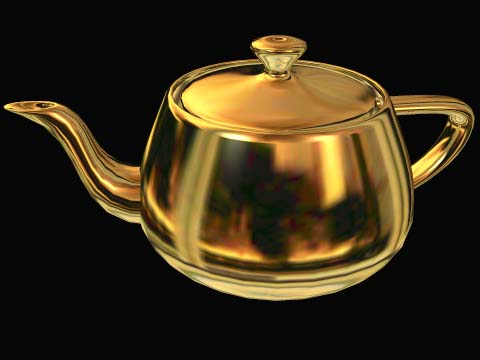
\includegraphics[height=80px]{images/teapot_texturing}
 \caption{Texturing}
 \end{subfigure}
 \begin{subfigure}{0.31\textwidth}
 \centering
 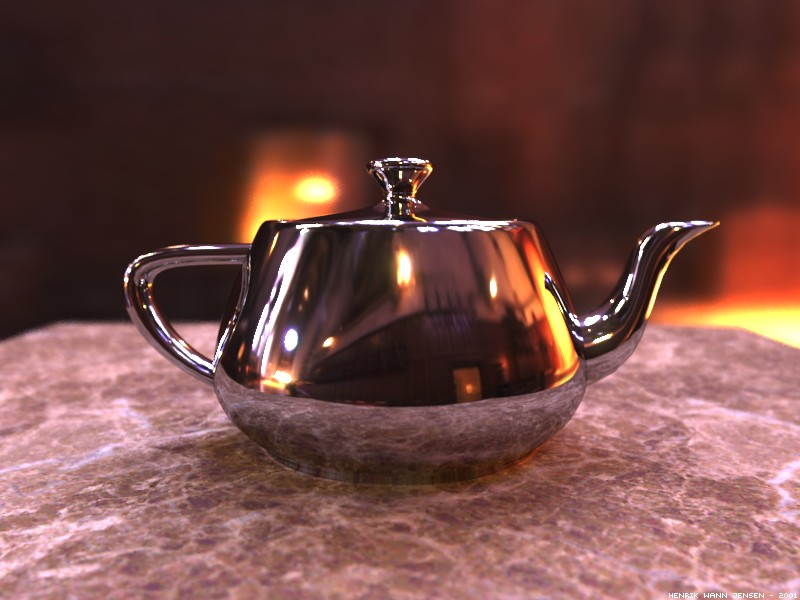
\includegraphics[height=80px]{images/teapot_rendering}
 \caption{Rendering}
 \end{subfigure}
\end{figure}

I will conclude the introductory presentation by showing the students some designs I've made in the past (see Fig \ref{fig:persPort}). This will give the students an idea of what one can do with the skills we learn.

\subsection{Practical Session - 2h}

This will be a hands-on session, where I will show the students how to create some basic 3D objects and put them together in a 3D scene. The students will try to replicate my steps on their computer, and I will pause if any student is left behind. The session will be highly interactive, and students will be able to suggest alternative ways of creating the objects.

The tasks that we will aim to do are:
\begin{itemize}
 \item Build a house (Fig \ref{1a}) - 40 min
 \item Animate the movement of a plane (Fig \ref{1b}) - 40 min
 \item Build realistic wine glasses (Fig \ref{1c})- 40 min
\end{itemize}

\begin{figure}[H]
 \begin{subfigure}{0.3\textwidth}
 \centering
  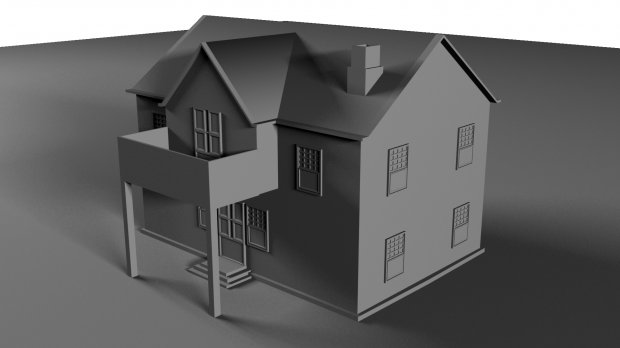
\includegraphics[height=80px]{images/house.jpg}
  \caption{House}
  \label{1a}
 \end{subfigure}
 \begin{subfigure}{0.3\textwidth}
 \centering
  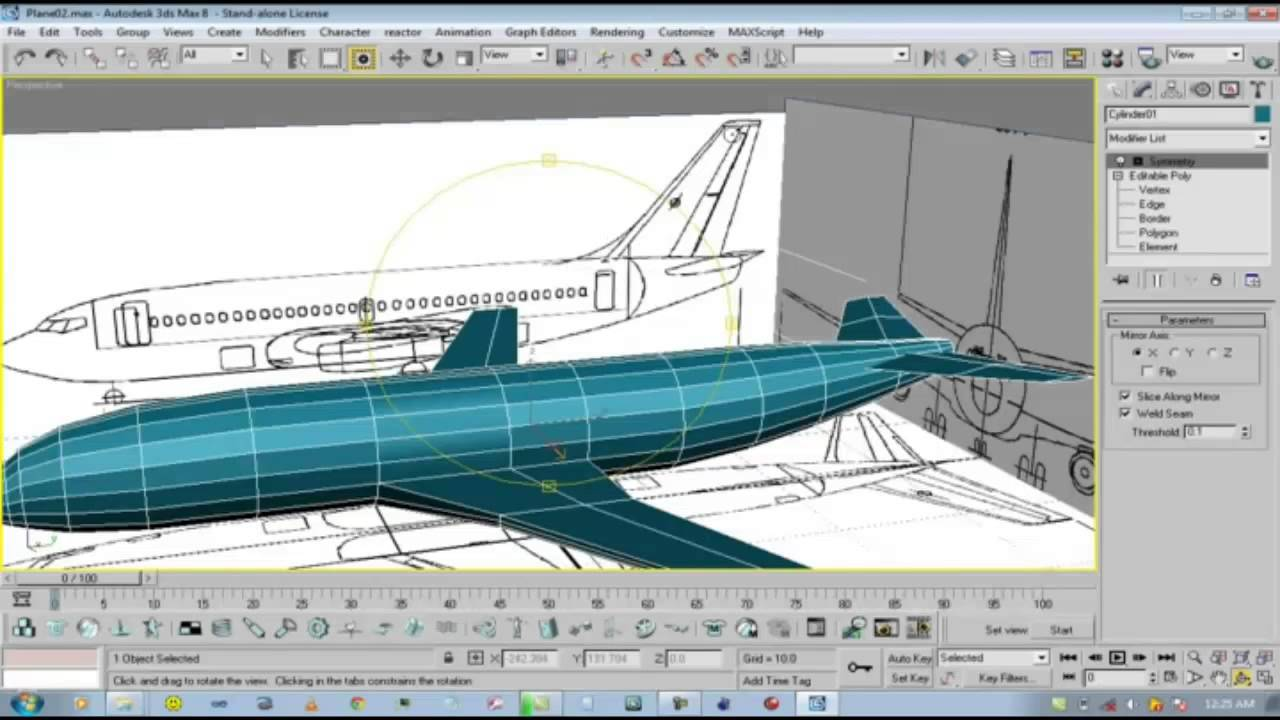
\includegraphics[height=80px, trim=0 0 200 0, clip]{images/plane.jpg}
  \caption{Plane}
  \label{1b}
 \end{subfigure}
 \begin{subfigure}{0.3\textwidth}
 \centering
  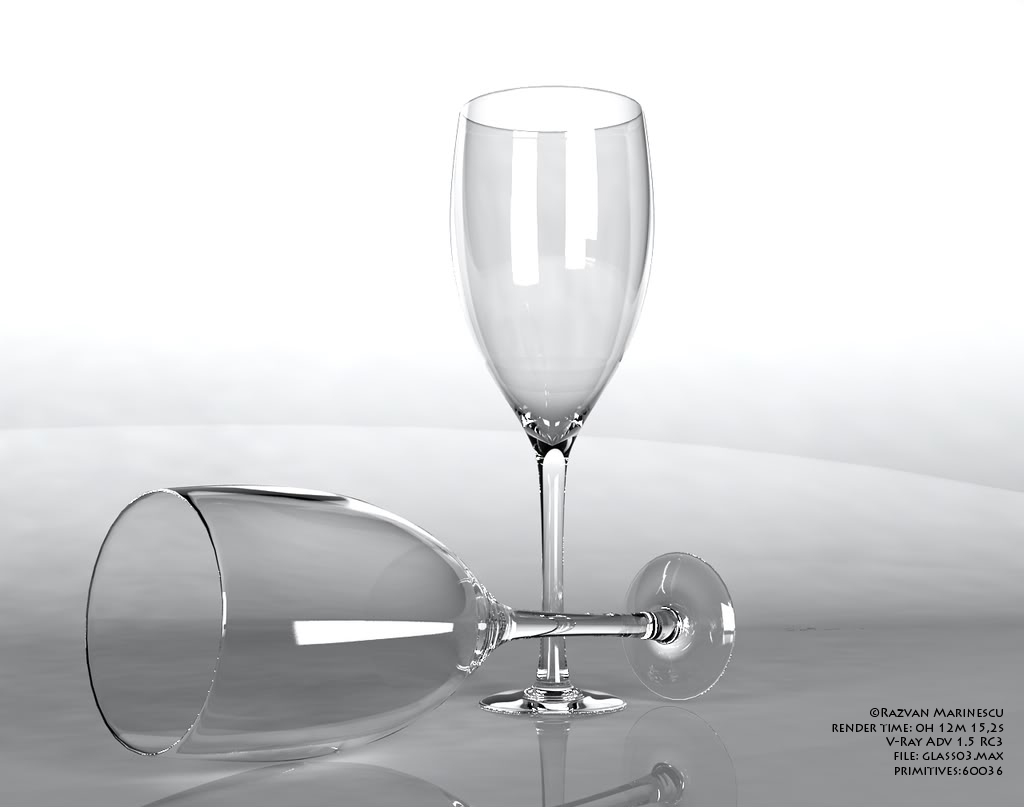
\includegraphics[height=80px]{images/glass03.jpg}
  \caption{Realistic wine glasses}
  \label{1c}
 \end{subfigure}
 \caption{Objects we will model in the practical session.}
\end{figure}



\subsection{Student-led Session - 1h}

The students will be grouped into teams and each team will be free to draw anything they like. At the end of the session, the teams will display their 3D images/animations in front of everyone else. Everyone will vote for the best 3D object/animation (self voting not permitted) and the winner team will be awarded a prize.


\section{Teaching Experience}

I have organised a 3-week course on this topic in 2013 at Imperial College (IC) London. I have also been a tutor for several programming and modelling courses:
\begin{itemize}
 \item Programming in Java/C++: Taught this for 1.5 years to first-year undergraduate students at IC. I was also responsible for marking their courseworks and going through the problems in the class.
 \item Computational Modelling in Medical Imaging: Lab helper for 1 term (3-4h/week). I was helping the students with any qestions regarding the coursework and with marking their courseworks.
\end{itemize}


\section{Personal Portofolio of 3D Computer Generated Graphics}

\begin{figure}[H]
 \begin{subfigure}{0.32\textwidth}
 \centering
 \vspace{1em}
  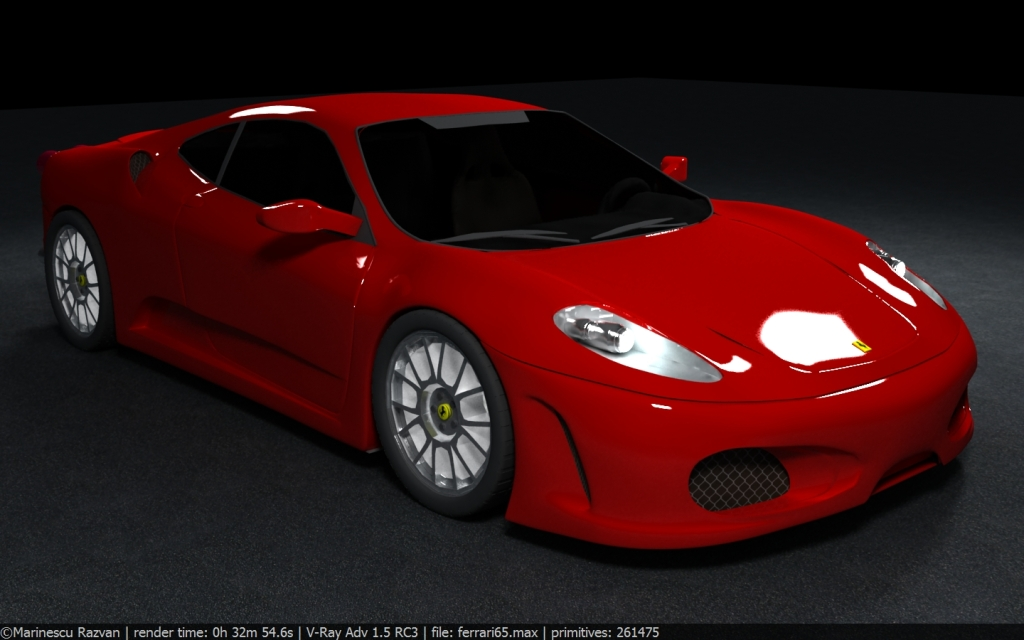
\includegraphics[width=\textwidth]{images/ferrari1440x900.jpg}
 \end{subfigure}
 \begin{subfigure}{0.32\textwidth}
 \centering
  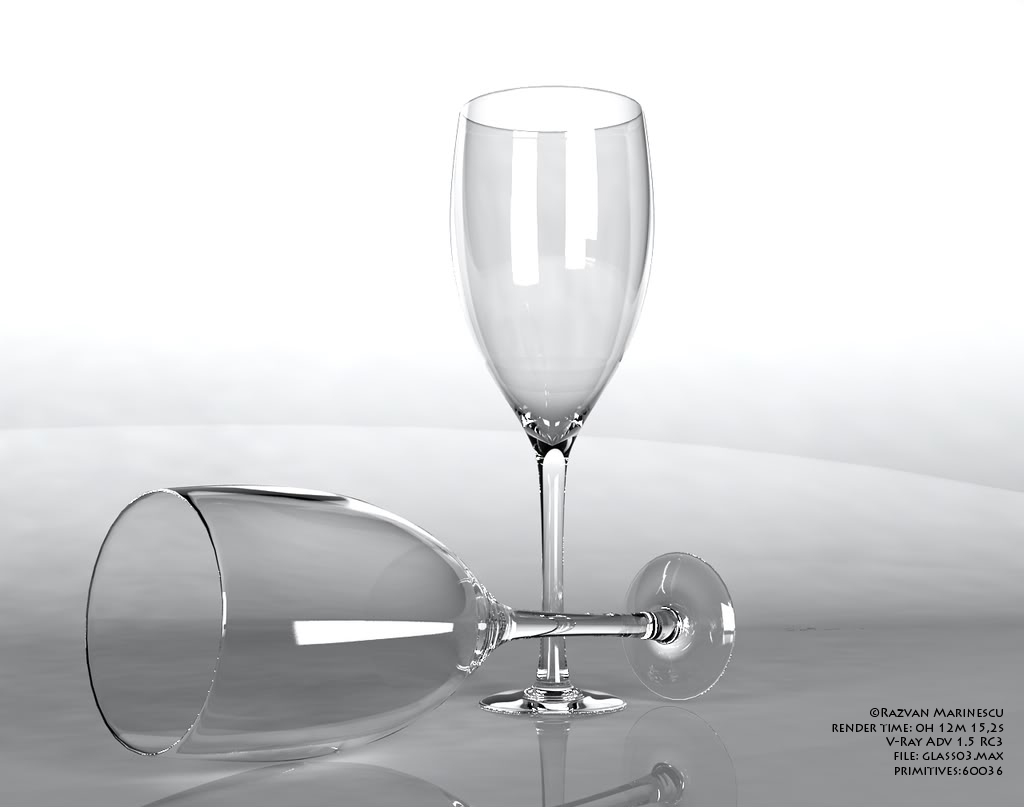
\includegraphics[width=\textwidth]{images/glass03.jpg}
 \end{subfigure}
 \begin{subfigure}{0.32\textwidth}
 \centering
  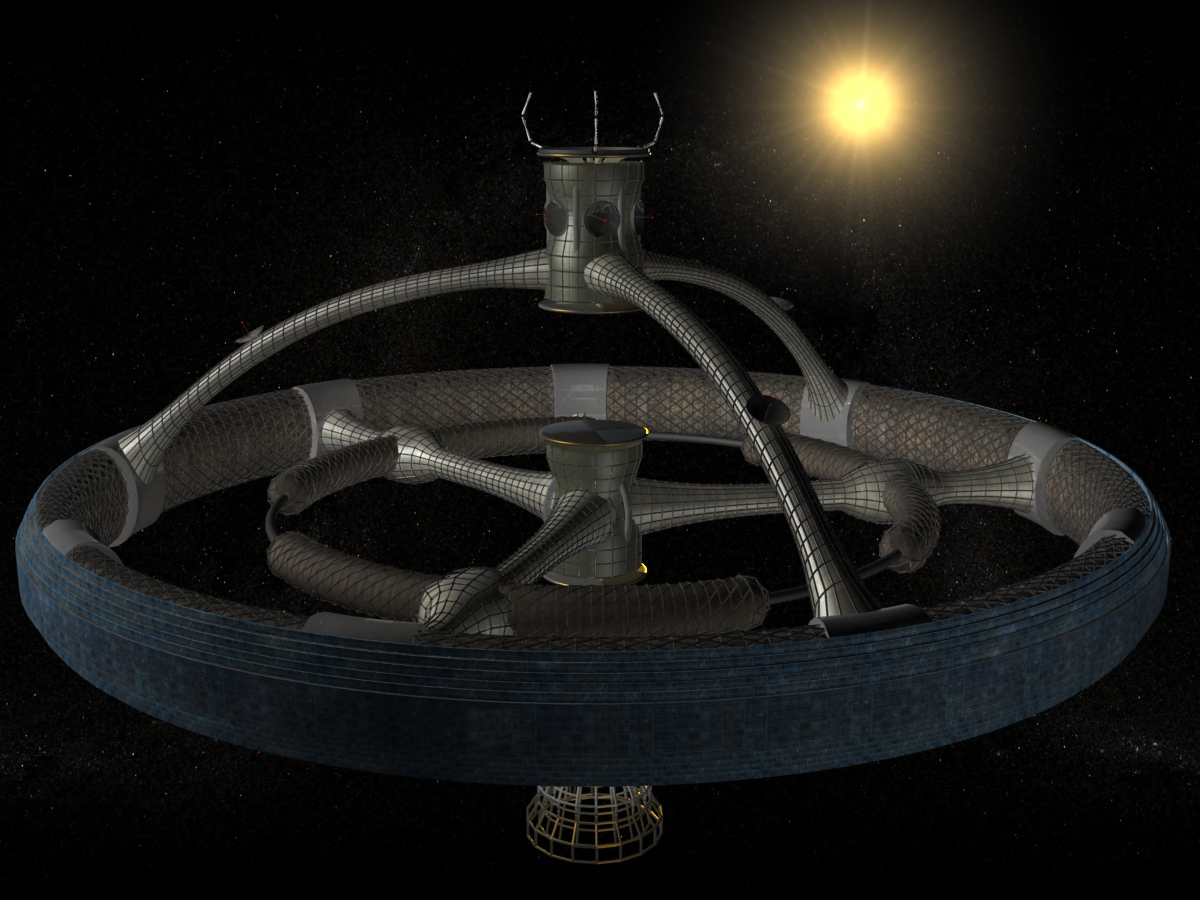
\includegraphics[width=\textwidth]{images/station02}
 \end{subfigure}
 
 \begin{subfigure}{0.32\textwidth}
 \centering
  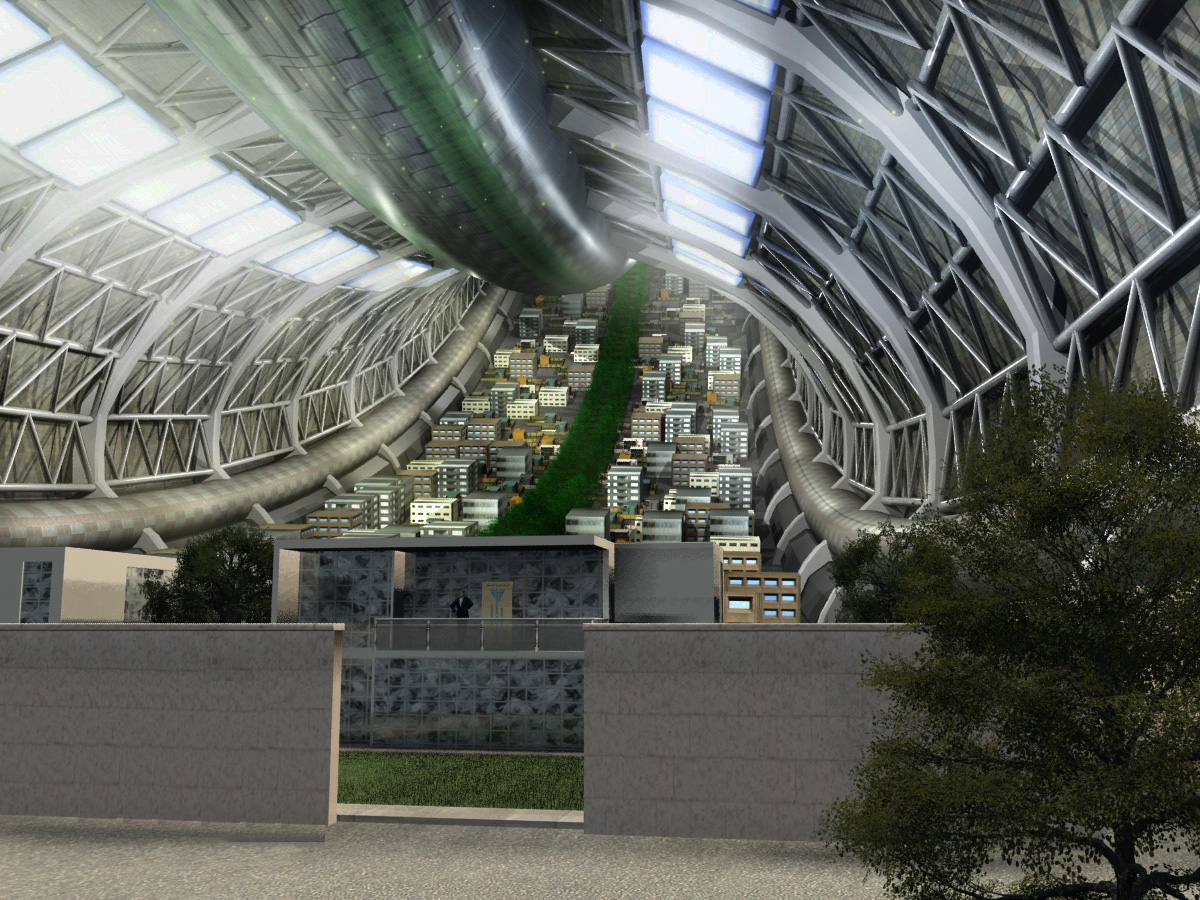
\includegraphics[width=\textwidth]{images/interior-final-nocharacters}
 \end{subfigure}
 \begin{subfigure}{0.32\textwidth}
 \centering
  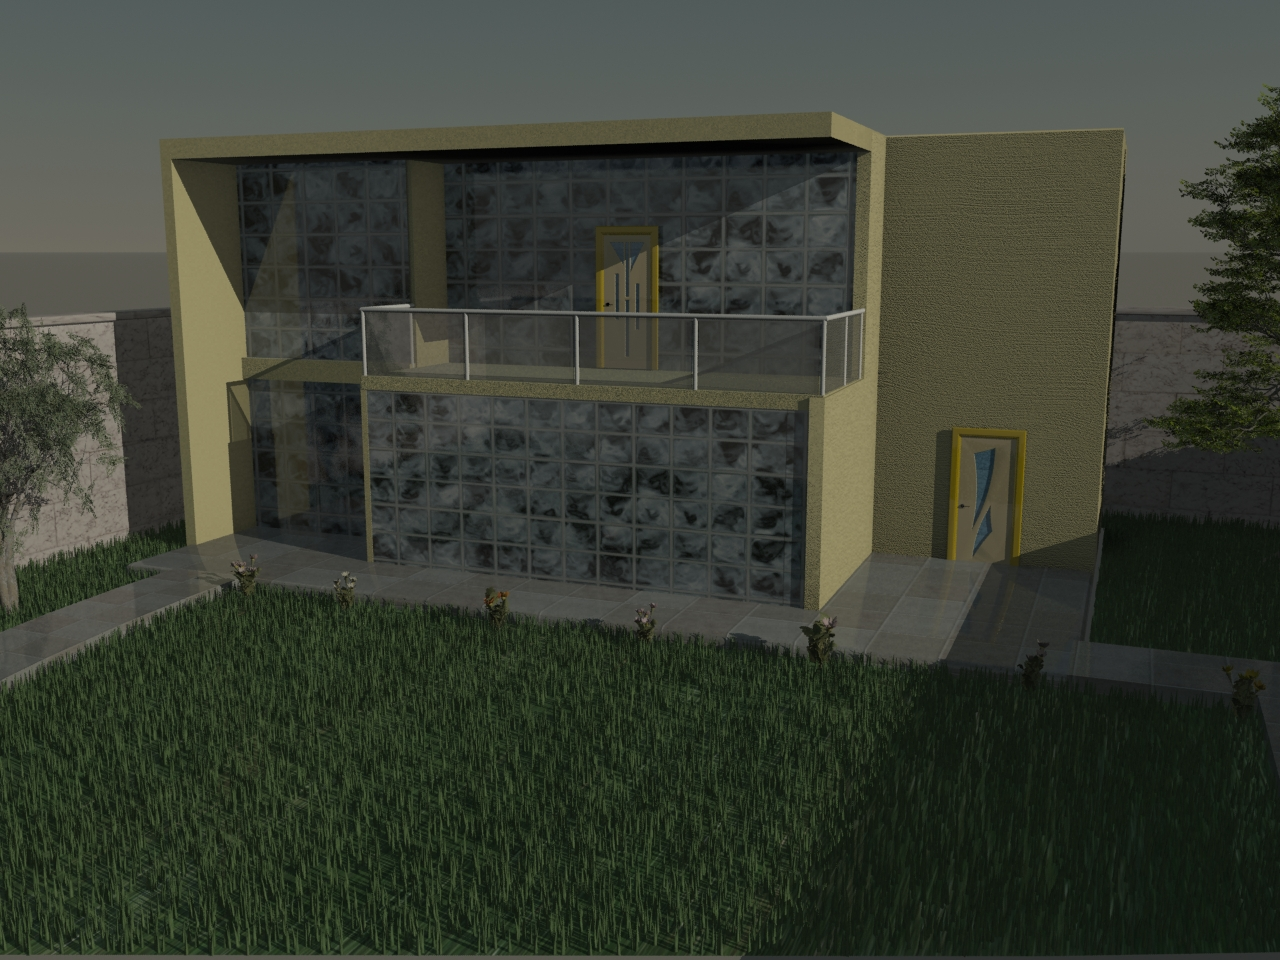
\includegraphics[width=\textwidth]{images/house2}
 \end{subfigure}
  \begin{subfigure}{0.32\textwidth}
 \centering
  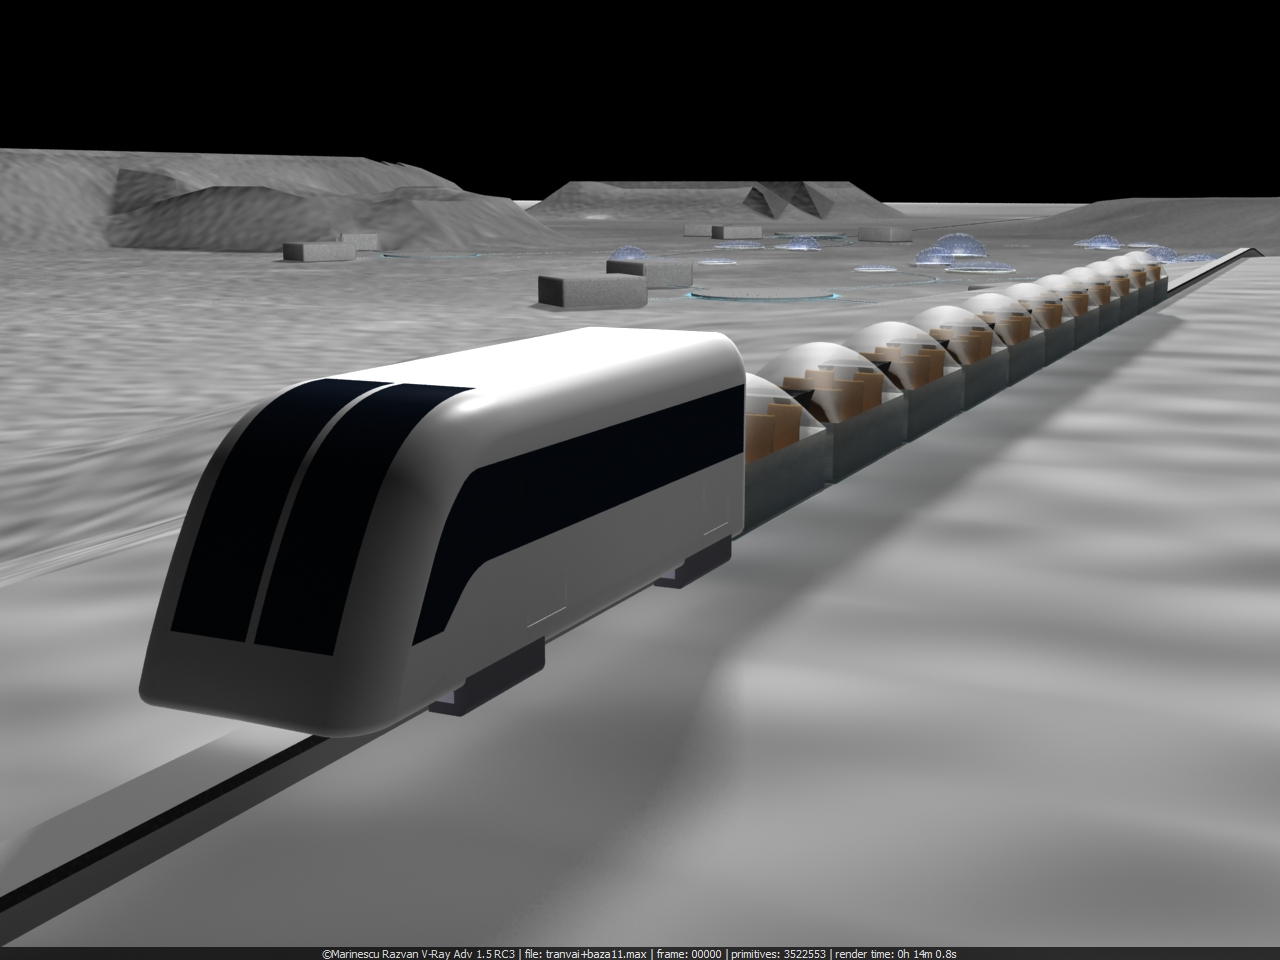
\includegraphics[width=\textwidth]{images/tranvai+baza-vray01.jpg}
 \end{subfigure}
 
 
 
 \caption{Collage of 3D computer-generated images that I've done so far.}
 \label{fig:persPort}
\end{figure}

\section{Materials Required}

\begin{itemize}
 \item One computer for every student with Autodesk 3d Studio Max already installed (I'm happy to install it beforehand)
 \item Projector + sound system for the PowerPoint presentation
\end{itemize}



\section{Availability and Time Slots}

I am available anytime apart from Tue 29 Aug and Wed 30 Aug. The course would ideally run for 3.5h, otherwise for a minimum of 3h. Any continuous time slot is ok.


\end{document}





















